\chapter{JDBGM}
En este capitulo describiremos el proyecto propuesto por este trabajo, empezaremos por recordar la problemática expuesta en el capitulo \fullref{capitulo:intro} pero de una manera mas técnica, además enmarcaremos el proyecto en un escenario mas especifico definiendo un lenguaje sobre el cual se desarrollara y los \dd a los que se les dará soporte, para luego exponer la solución propuesta.

\section{El problema}
Como empezamos a describir en la introducción del capitulo \ref{capitulo:intro} la dificultad que encontramos al usar motores de bases de datos en el desarrollo de sistemas informáticos se traduce en problemas de mantenibilidad y portabilidad, veamos estos dos puntos por separado:
\begin{itemize}
\item Problemas en la portabilidad: Al utilizar un motor\footnote{Hablando de motores de bases de datos} en particular nos atamos en mayor o menor medida al uso de este según como hayamos diseñado el sistema, el mayor problema se traduce en las diferentes sintaxis para SQL que define cada \dd culpa de ello es muy probable que una sentencia valida para un motor no lo sea para otro, por lo tanto a la hora de querer migrar desde un motor a otro e inclusive a una versión mas nueva del mismo motor es necesario  ``actualizar'' las sentencias para que se apeguen a la sintaxis del motor al que se pretende migrar. Además como parte de su sintaxis particular cada \dd define sus propios tipos de datos lo que añade un poco mas de dificultad al proceso de cambio o migración desde un motor a otro.  
\item  Problemas en el mantenimiento: al utilizar bases de datos es importante como se diseña el acceso y manejo de los \dd, hay que tener en cuenta las siguientes cuestiones: quien se tiene que hacer cargo de la persistencia de los datos? El programa tiene que conocer los datos o mas bien como obtener los datos? Estas cuestiones no son nuevas y se solucionan en parte siguiendo patrones de diseño. Un ejemplo mas conciso de esto lo podemos ver cuando se esta diseñando un modulo de un sistema que precisa persistir ciertos datos en una BD, la pregunta que hay que hacerse es quien debería hacerse cargo de realizar esta persistencia? Si lo hace el modulo en si nos encontraríamos con accesos a la base de datos mezclados con la lógica de negocio del modulo además estos accesos implican que el modulo debe conocer como conectarse con la base de datos y de que modo se deben enviar y recibir los datos, con lo que nuestro modulo	perdería cohesión y ganaría complejidad derivando todo esto en una mayor dificultad en el mantenimiento.
\end{itemize}
Estos dos puntos están fuertemente relacionados pues la mantenibilidad del software esta muy ligada a la portabilidad y viceversa, esto por que la portabilidad hace a la mantenibilidad, pero cuando hablamos de que el software sea mantenible estamos hablando de muchos aspectos mas. Este trabajo esta centrado en el uso de la base de datos y como afecta esto a estos dos aspectos. Como ya se dijo es de buena practica el uso de patrones de diseño, así que en la sección siguiente veamos que es esto y como nos va a ayudar a encontrar una base para el proyecto. 
\section{Patrones de diseño}
Un patrón de diseño es una solución genérica y reusable  a un problema que ocurre de manera frecuente en un contexto dado. Un patrón de diseño no es un diseño terminado que pueda ser transformado directamente en código es mas bien una guía que indica como resolver un problema en determinados escenarios. Así los patrones de diseño son buenas costumbres que uno mismo debe implementar en la aplicación a desarrollar y en este mismo sentido son recomendaciones a tener en cuenta y no obligaciones\cite{Metsker:2002:DPJ}. Además es importante notar que el uso de patrones no garantiza éxito a la hora de diseñar. La descripción de un patrón indica cuando este puede ser aplicable, pero solo la experiencia nos hará comprender cuando el uso de un patrón de diseño en particular mejorara el diseño del software\cite{java:patrones}.


Entonces por que tener en cuenta a los patrones?
\begin{itemize}
\item Han sido provados. Los patrones reflejan la experiencia, conocimiento y perspectiva de desarrolladores quienes han aplicado satisfactoriamente estos patrones en su propio trabajo.

\item Son reusables. Los patrones proveen soluciones ya descubiertas que pueden ser aplicadas a diferentes problemas.

\item Son expresivos. Los patrones proveen un vocabulario común de soluciones que pueden expresar soluciones extensas de manera concisa.
%They are expressive. Patterns provide a common vocabulary of solutions that can express large solutions succinctly.
\end{itemize}
Existe mucha teoría sobre los patrones pero en este trabajo no nos interesa ahondar sobre ellos si no que interesaba introducir el concepto al lector para conocer un patrón que servirá de base para el desarrollo de \jj
\subsection{Data Acces Object}
Antes de describir este patrón tenemos que ubicarnos en un \textbf{contexto}, al acceso a los datos depende de la fuente de datos con la que se este trabajando. El acceso a almacenamiento persistente de datos, tal como una base de datos, varia fuertemente dependiendo del tipo de almacenamiento (BD relacionales, BD orientadas a objetos, archivos planos, etc) y de la implementación de un proveedor en particular.

El \textbf{problema} se da por que en cierto punto las aplicaciones necesitan persistir sus datos. Para muchas aplicaciones, la persistencia de los datos es implementada mediante diferentes mecanismos y hay marcadas diferencias en las API's usadas para acceder a estos diferentes mecanismos. Otras aplicaciones quizás necesite acceder a datos almacenados en diferentes sistemas muy distintos del cual se esta trabajando los cuales exigen utilizar sus APIs las cuales usualmente son propietarias. Esta disparidad entre las diferentes fuentes de datos produce desafíos en el diseño y además crea una potencial dependencia directa entre el código de la aplicación y el código de acceso a los datos. Dicha dependencia en el código de los componentes de la aplicación vuelve tediosa y dificultosa la migración desde un tipo de persistencia de datos a otra pues cuando cambia la fuente de datos el componente debe ser modificado para poder manejar la nueva fuente de datos.

La \textbf{solución} a este problema viene por usar un DAO (Data Acces Object) para abstraer y encapsular todos los accesos a la fuente de datos. DAO maneja la conexión con la fuente de datos para obtener y almacenar los datos.

EL DAO implementa los mecanismos de acceso necesarios para trabajar con la fuente de datos, esta fuente de datos puede ser un almacén de persistencia de cualquier tipo como por ejemplo un RDBMS, un servicio externo, un repositorio o incluso archivos xml. El componente del negocio (aquel que trabaja con la lógica del negocio) que se apoya en el DAO accede a la interfaz simplificada que este brinda para sus clientes. El DAO oculta completamente los detalles de la implementación de la fuente de datos a sus clientes y como la interfaz expuesta a los clientes del DAO no cambia cuando cambia la implementación de la fuente de datos este patrón permite que el DAO se adapte a diferentes esquemas de almacenamiento sin afectar sus clientes o componentes del negocio. Esencialmente el DAO actua como un adaptador entre el componente y la estructura de la fuente de datos.

% The DAO completely hides the data source implementation details from its clients. Because the interface exposed by the DAO to clients does not change when the underlying data source implementation changes, this pattern allows the DAO to adapt to different storage schemes without affecting its clients or business components. Essentially, the DAO acts as an adapter between the component and the data source.

La figura \ref{fig:dao-structure} muestra un diagrama de clases que muestras las relaciones en el patrón DAO.  

\begin{figure}
  \centering
    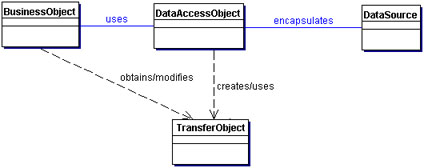
\includegraphics[width=0.6\textwidth]{figuras/dao-structure.jpg}
  \caption{Data Acces Object}
  \label{fig:dao-structure}
\end{figure}

Para finalizar nombremos las consecuencias de usar este patrón:
\begin{itemize}
\item Provee transparencia. El acceso a la fuente de datos es transparente pues los detalles de la implementación estan ocultos en el DAO. 


\item Facilita la migración.%Enables Easier Migration A layer of DAOs makes it easier for an application to migrate to a different database implementation. The business objects have no knowledge of the underlying data implementation. Thus, the migration involves changes only to the DAO layer. Further, if employing a factory strategy, it is possible to provide a concrete factory implementation for each underlying storage implementation. In this case, migrating to a different storage implementation means providing a new factory implementation to the application. 

\item Reduce la complejidad del código en los objetos que manejan la lógica del negocio. %Reduces Code Complexity in Business ObjectsBecause the DAOs manage all the data access complexities, it simplifies the code in the business objects and other data clients that use the DAOs. All implementation-related code (such as SQL statements) is contained in the DAO and not in the business object. This improves code readability and development productivity. 

\item Centraliza todo el acceso a los datos en una capa separada. %Centralizes All Data Access into a Separate Layer Because all data access operations are now delegated to the DAOs, the separate data access layer can be viewed as the layer that can isolate the rest of the application from the data access implementation. This centralization makes the application easier to maintain and manage. 

\item 
Not Useful for Container-Managed Persistence
% Because the EJB container manages entity beans with container-managed persistence (CMP), the container automatically services all persistent storage access. Applications using container-managed entity beans do not need a DAO layer, sjdbcjdbcince the application server transparently provides this functionality. However, DAOs are still useful when a combination of CMP (for entity beans) and BMP (for session beans, servlets) is required. 


\item Agrega una capa extra, la cual debe ser diseñada e implementada para beneficiarse del uso de este patrón. %Adds Extra Layer The DAOs create an additional layer of objects between the data client and the data source that need to be designed and implemented to leverage the benefits of this pattern. But the benefit realized by choosing this approach pays off for the additional effort. 

\item Necesita diseño de jerarquía de clases, que implica otro esfuerzo extra. %Needs Class Hierarchy Design When using a factory strategy, the hierarchy of concrete factories and the hierarchy of concrete products produced by the factories need to be designed and implemented. This additional effort needs to be considered if there is sufficient justification warranting such flexibility. This increases the complexity of the design. However, you can choose to implement the factory strategy starting with the Factory Method pattern first, and then move towards the Abstract Factory if necessary.

\end{itemize}


\section{La solucion propuesta: \jj}
Después de conocer el patrón nos damos cuenta que el problema al que apunta la tesis es común y a veces inevitable, entonces por que desarrollar este proyecto? Pues para aquellos desarrollos donde el patrón sea aplicable. Además debemos recordar que el presente trabajo esta acotado a Java y bases de datos relacionales, lo que limita en cierto modo a la definición dada para DAO en el sentido de que no tenemos en cuenta otros tipo de mecanismos de persistencia de datos. Entonces veamos específicamente de que trata el proyecto.

Para trabajar con \dd Java provee la API JDBC\cite{java:jdbc} que según su documentación provee un medio para acceder virtualmente a cualquier tipo de datos tabulares. JDBC es usado para invocar comandos SQL directamente aunque también fue diseñado para ser la base sobre la cual se construyen herramientas e interfaces alternativas mas amigables con el ``usuario'' en el sentido que se puede construir un API mas entendible o conveniente que es en el fondo traducida para usar JDBC. Como en nuestro proyecto queremos ocultar el acceso explicito a una base de datos no podemos usar directamente JDBC pues al usarlo directamente necesitaríamos explicitar la conexión con el motor de la base de datos
